\documentclass[11pt,letter]{article}\usepackage[]{graphicx}\usepackage[]{color}
%% maxwidth is the original width if it is less than linewidth
%% otherwise use linewidth (to make sure the graphics do not exceed the margin)
\makeatletter
\def\maxwidth{ %
  \ifdim\Gin@nat@width>\linewidth
    \linewidth
  \else
    \Gin@nat@width
  \fi
}
\makeatother

\definecolor{fgcolor}{rgb}{0.345, 0.345, 0.345}
\newcommand{\hlnum}[1]{\textcolor[rgb]{0.686,0.059,0.569}{#1}}%
\newcommand{\hlstr}[1]{\textcolor[rgb]{0.192,0.494,0.8}{#1}}%
\newcommand{\hlcom}[1]{\textcolor[rgb]{0.678,0.584,0.686}{\textit{#1}}}%
\newcommand{\hlopt}[1]{\textcolor[rgb]{0,0,0}{#1}}%
\newcommand{\hlstd}[1]{\textcolor[rgb]{0.345,0.345,0.345}{#1}}%
\newcommand{\hlkwa}[1]{\textcolor[rgb]{0.161,0.373,0.58}{\textbf{#1}}}%
\newcommand{\hlkwb}[1]{\textcolor[rgb]{0.69,0.353,0.396}{#1}}%
\newcommand{\hlkwc}[1]{\textcolor[rgb]{0.333,0.667,0.333}{#1}}%
\newcommand{\hlkwd}[1]{\textcolor[rgb]{0.737,0.353,0.396}{\textbf{#1}}}%

\usepackage{framed}
\makeatletter
\newenvironment{kframe}{%
 \def\at@end@of@kframe{}%
 \ifinner\ifhmode%
  \def\at@end@of@kframe{\end{minipage}}%
  \begin{minipage}{\columnwidth}%
 \fi\fi%
 \def\FrameCommand##1{\hskip\@totalleftmargin \hskip-\fboxsep
 \colorbox{shadecolor}{##1}\hskip-\fboxsep
     % There is no \\@totalrightmargin, so:
     \hskip-\linewidth \hskip-\@totalleftmargin \hskip\columnwidth}%
 \MakeFramed {\advance\hsize-\width
   \@totalleftmargin\z@ \linewidth\hsize
   \@setminipage}}%
 {\par\unskip\endMakeFramed%
 \at@end@of@kframe}
\makeatother

\definecolor{shadecolor}{rgb}{.97, .97, .97}
\definecolor{messagecolor}{rgb}{0, 0, 0}
\definecolor{warningcolor}{rgb}{1, 0, 1}
\definecolor{errorcolor}{rgb}{1, 0, 0}
\newenvironment{knitrout}{}{} % an empty environment to be redefined in TeX

\usepackage{alltt}    
%\usepackage[latin1]{inputenc}
\usepackage[parfill]{parskip} % Activate to begin paragraphs with an empty line rather than an indent
\usepackage{amsmath,amsthm,amssymb,bbm} %math stuff
\usepackage{ctable}
\usepackage{placeins} % FloatBarrier
\usepackage{fancyhdr}
\usepackage{lastpage}
\usepackage{float}    % for fig.pos='H'
\usepackage{rotfloat} % for sidewaysfigure
%\usepackage{subfig}   % for subfigure
\usepackage{subcaption}  % an alternative package for sub figures
\newcommand{\subfloat}[2][need a sub-caption]{\subcaptionbox{#1}{#2}}
\usepackage{comment}
\usepackage[round]{natbib}   % omit 'round' option if you prefer square brackets
\bibliographystyle{plainnat}
\usepackage{setspace} %Spacing
\usepackage{graphicx,graphics}
\usepackage{booktabs,tabularx}
\usepackage{enumerate}
\usepackage{makecell}
\usepackage{xfrac}
\usepackage{color, colortbl, xcolor}
\usepackage{booktabs,dcolumn} % for use with texreg in R
\usepackage[pagebackref=true,bookmarks]{hyperref}
\hypersetup{
    unicode=false,          
    pdftoolbar=true,        
    pdfmenubar=true,        
    pdffitwindow=false,     % window fit to page when opened
    pdfstartview={FitH},    % fits the width of the page to the window
    pdftitle={006-Sensitivity Analysis of One Parameter},    % title
    pdfauthor={SRB},     % author
    pdfsubject={Subject},   % subject of the document
    pdfcreator={SRB},   % creator of the document
    pdfproducer={SRB}, % producer of the document
    pdfkeywords={}, % list of keywords
    pdfnewwindow=true,      % links in new window
    colorlinks=true,       % false: boxed links; true: colored links
    linkcolor=red,          % color of internal links (change box color with linkbordercolor)
    citecolor=blue,        % color of links to bibliography
    filecolor=black,      % color of file links
    urlcolor=cyan           % color of external links
}

% my commands
\newcommand{\tm}[1]{\textrm{#1}}


% fancy header commands
\renewcommand{\headrulewidth}{0.0pt}
\renewcommand{\footrulewidth}{0.0pt}
\setlength{\textheight}{9.00in}
\setlength{\textwidth}{7.00in}
\setlength{\topmargin}{-0.5in}
\setlength{\evensidemargin}{-0.25in}
\setlength{\oddsidemargin}{-0.25in}
\renewcommand{\baselinestretch}{1.2}
\makeatletter
\makeatother
\lfoot{} \cfoot{ } \rfoot{{\small{\em Page \thepage \ of \pageref{LastPage}}}}
\IfFileExists{upquote.sty}{\usepackage{upquote}}{}
\begin{document}
\pagestyle{fancy}

\title{007-Sensitivity Analysis of Many Paramters}
\author{Clustering Gene Expression Data}
\maketitle







\begin{abstract}
DNA microarrays may be used to characterize the molecular variations among tumors by monitoring gene expression profiles on a genomic scale. This may lead to a finer and more reliable classification of tumors, and to the identification of marker genes that distinguish among these classes. Eventual clinical implications include an improved ability to understand and predict cancer survival~\citep{cluster}. Therefore, a common task is to determine whether or not gene expression data can reliably identify or classify different types of a disease. We consider gene expression data from patients with acute lymphoblastic leukemia (ALL) that were investigated using HGU95AV2 Affymetrix GeneChip arrays~\citep{chiaretti2004gene}. The data consist of 128 patients with 12,625 genes. A number of additional covariates are available such as the type and stage of the disease; ``B'' indicates B-cell ALL, while a ``T'' indicates T-cell ALL. Several clustering procedures require user imputs such as the type of clustering and the number of clusters. Pre-filtering the data based on the most variable genes can also lead to increased power. We are interested in the effect these parameters have on the clustering results. Here I provide an illustration of performing such a task in an efficient and reproducible way using the function \texttt{knitr::knit\_expand}.
\end{abstract}


\tableofcontents





\newpage
\section{Method: ward.D, Filter: 95\%, Groups: 2}



\begin{knitrout}
\definecolor{shadecolor}{rgb}{0.969, 0.969, 0.969}\color{fgcolor}\begin{kframe}
\begin{alltt}
\hlkwd{dim}\hlstd{(dat.filter)}
\end{alltt}
\begin{verbatim}
## [1] 632 128
\end{verbatim}
\begin{alltt}
\hlkwd{table}\hlstd{(groups, cl)}
\end{alltt}
\begin{verbatim}
##       cl
## groups  B  T
##      1 95  0
##      2  0 33
\end{verbatim}
\begin{alltt}
\hlkwd{fisher.test}\hlstd{(groups, cl)}\hlopt{$}\hlstd{p.value}
\end{alltt}
\begin{verbatim}
## [1] 2.3e-31
\end{verbatim}
\end{kframe}
\end{knitrout}

\begin{knitrout}
\definecolor{shadecolor}{rgb}{0.969, 0.969, 0.969}\color{fgcolor}\begin{figure}[H]
\subfloat[Dendogram \label{fig:hclust-plot-ward.D-95-21}]{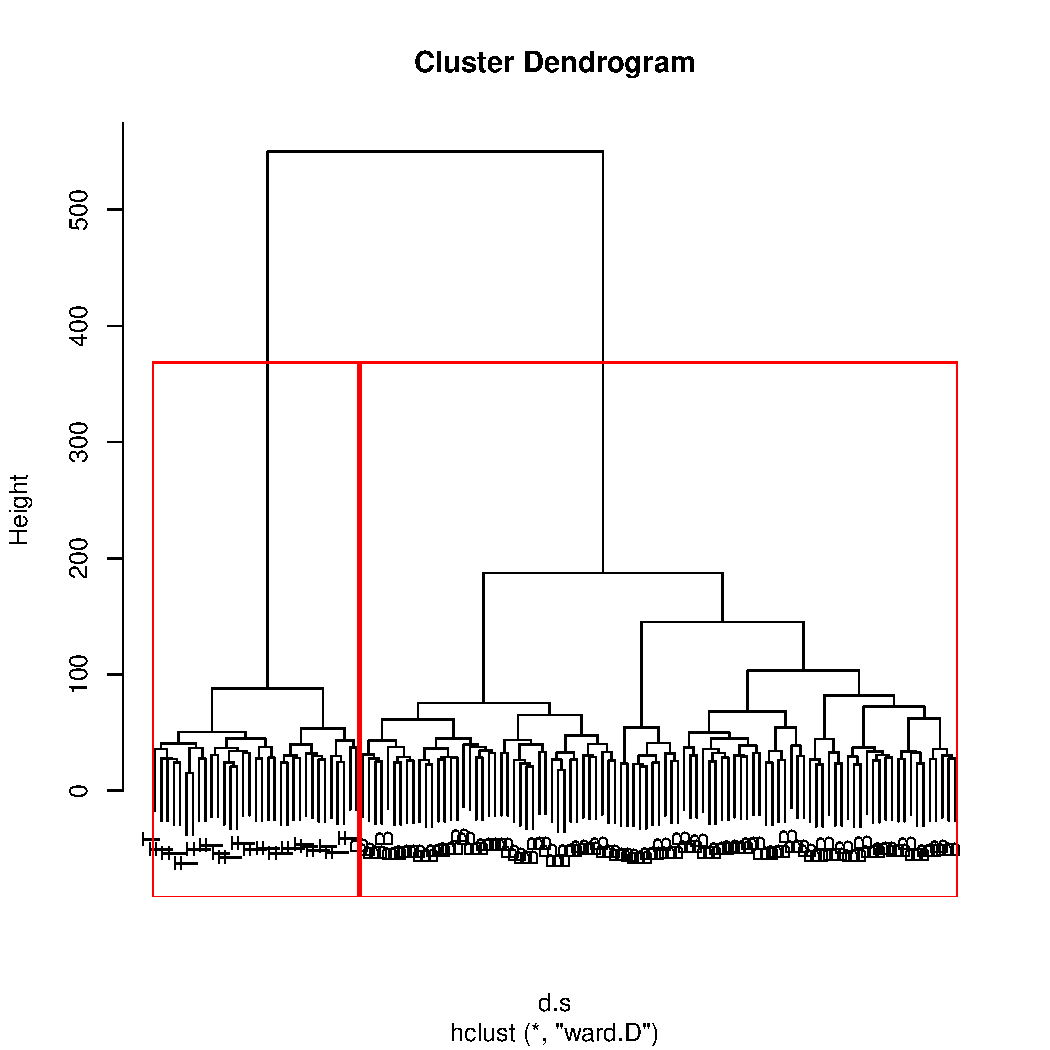
\includegraphics[width=.49\linewidth]{figure/hclust-plot-ward_D-95-2-1} }
\subfloat[Distance Matrix\label{fig:hclust-plot-ward.D-95-22}]{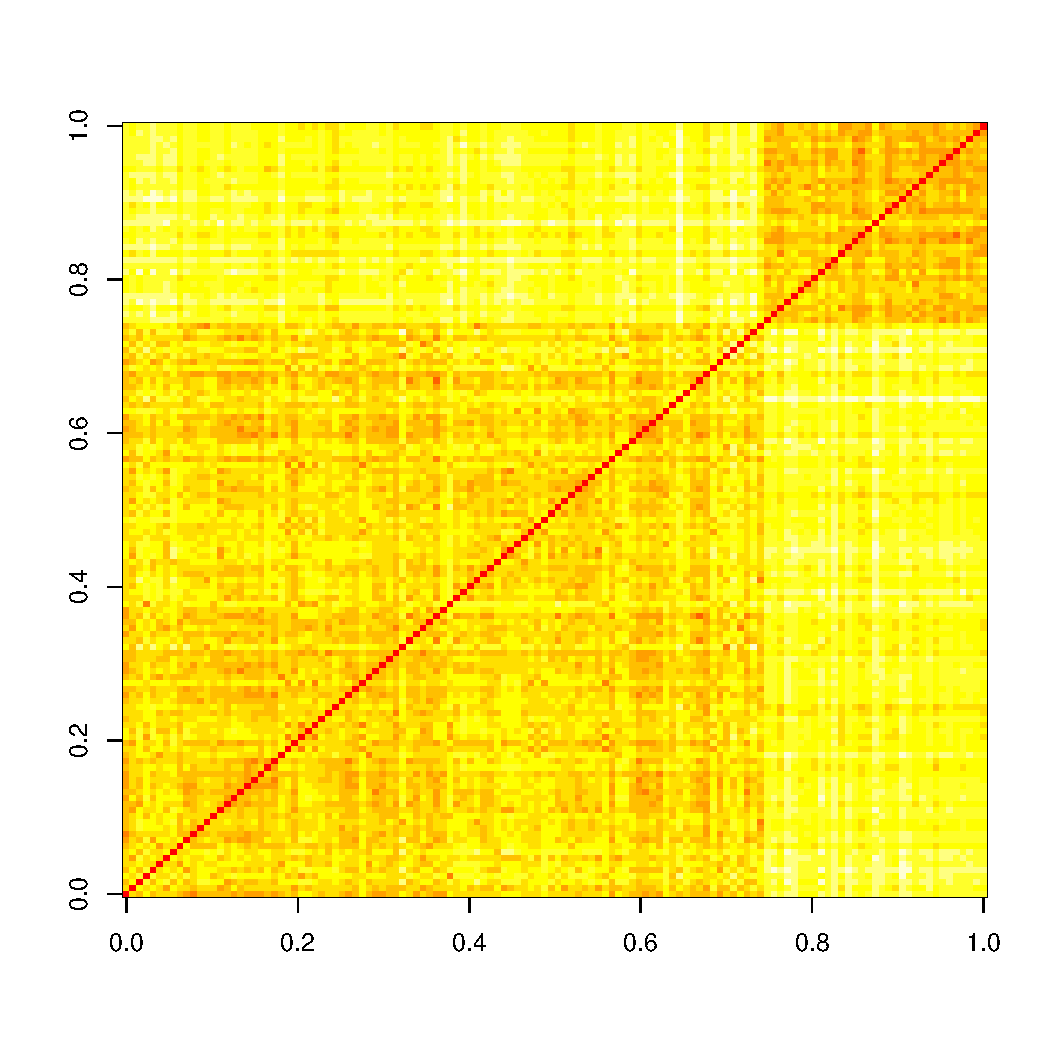
\includegraphics[width=.49\linewidth]{figure/hclust-plot-ward_D-95-2-2} }\caption[based on Method]{based on Method: ward.D, Filter: 95\%, Groups: 2}\label{fig:hclust-plot-ward.D-95-2}
\end{figure}


\end{knitrout}


\begin{knitrout}
\definecolor{shadecolor}{rgb}{0.969, 0.969, 0.969}\color{fgcolor}\begin{figure}[H]

{\centering 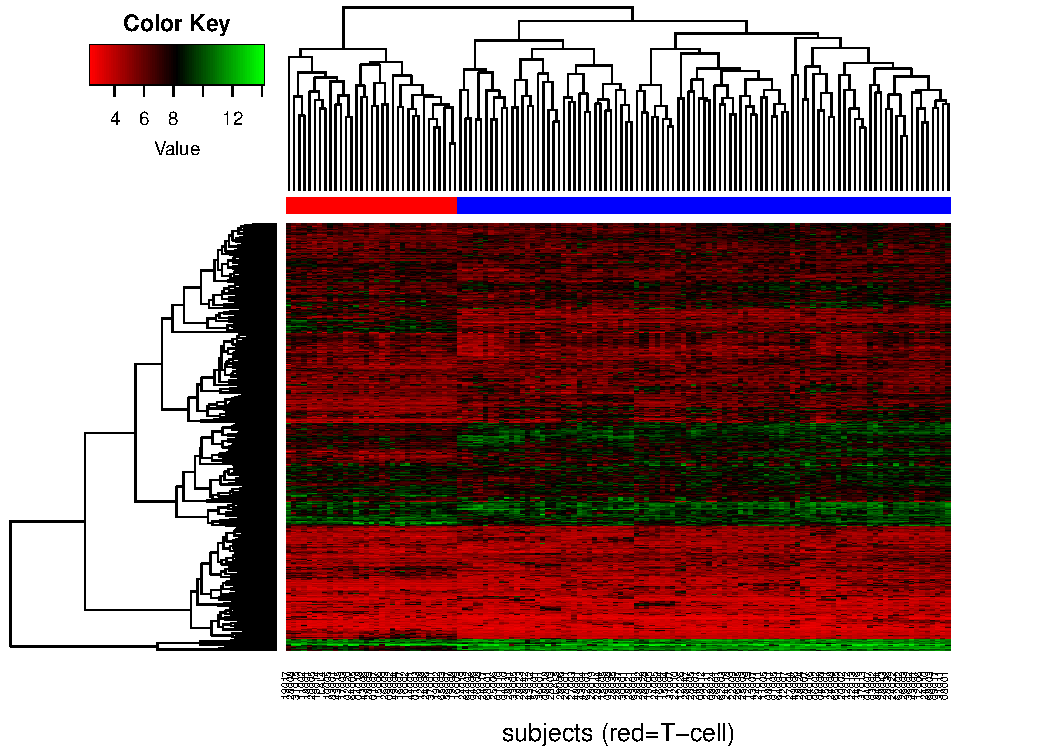
\includegraphics[width=\maxwidth]{figure/heatmap-ward_D-95-2-1} 

}

\caption[Heatmap of Gene expression values for genes that survived a filter of 95\%]{Heatmap of Gene expression values for genes that survived a filter of 95\%}\label{fig:heatmap-ward.D-95-2}
\end{figure}


\end{knitrout}


\newpage
\section{Method: single, Filter: 95\%, Groups: 2}



\begin{knitrout}
\definecolor{shadecolor}{rgb}{0.969, 0.969, 0.969}\color{fgcolor}\begin{kframe}
\begin{alltt}
\hlkwd{dim}\hlstd{(dat.filter)}
\end{alltt}
\begin{verbatim}
## [1] 632 128
\end{verbatim}
\begin{alltt}
\hlkwd{table}\hlstd{(groups, cl)}
\end{alltt}
\begin{verbatim}
##       cl
## groups  B  T
##      1 95 32
##      2  0  1
\end{verbatim}
\begin{alltt}
\hlkwd{fisher.test}\hlstd{(groups, cl)}\hlopt{$}\hlstd{p.value}
\end{alltt}
\begin{verbatim}
## [1] 0.26
\end{verbatim}
\end{kframe}
\end{knitrout}

\begin{knitrout}
\definecolor{shadecolor}{rgb}{0.969, 0.969, 0.969}\color{fgcolor}\begin{figure}[H]
\subfloat[Dendogram \label{fig:hclust-plot-single-95-21}]{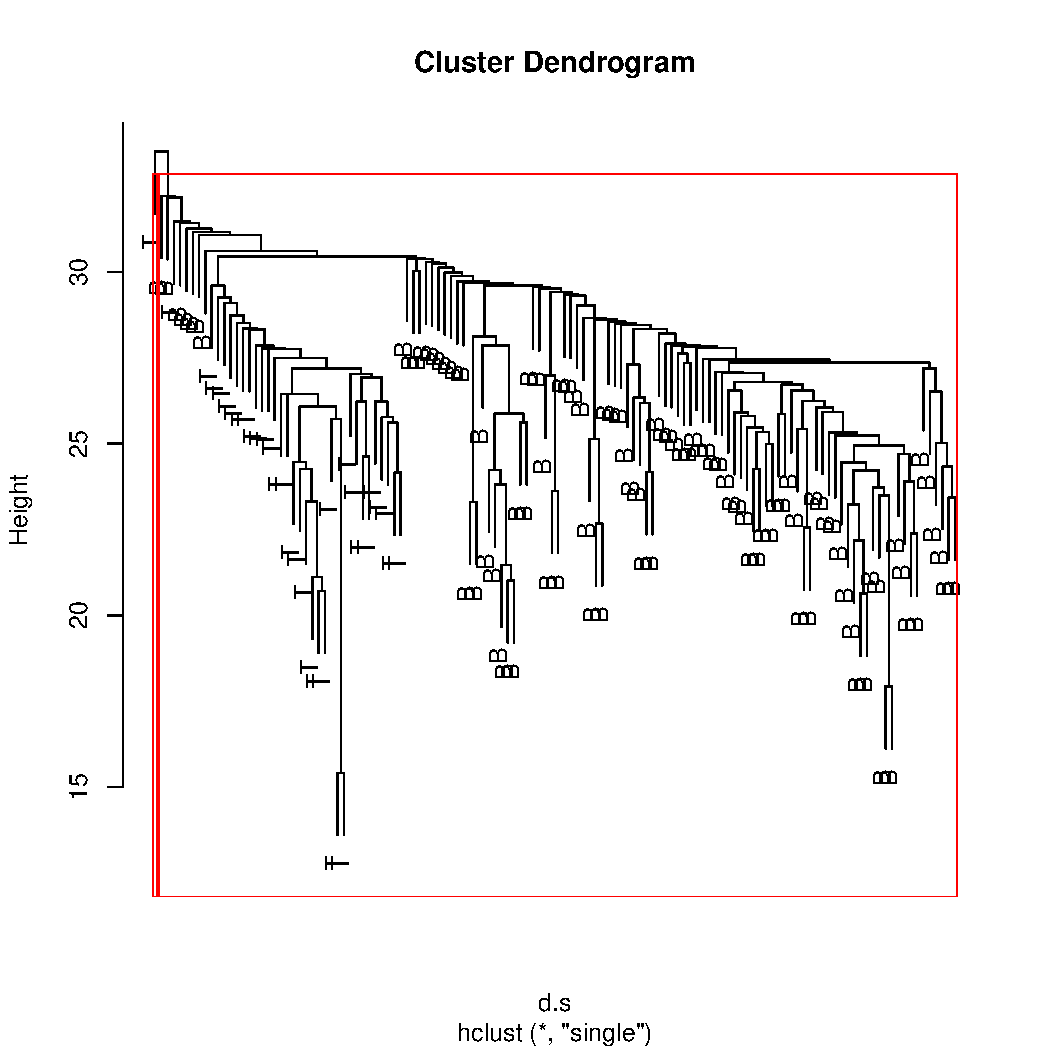
\includegraphics[width=.49\linewidth]{figure/hclust-plot-single-95-2-1} }
\subfloat[Distance Matrix\label{fig:hclust-plot-single-95-22}]{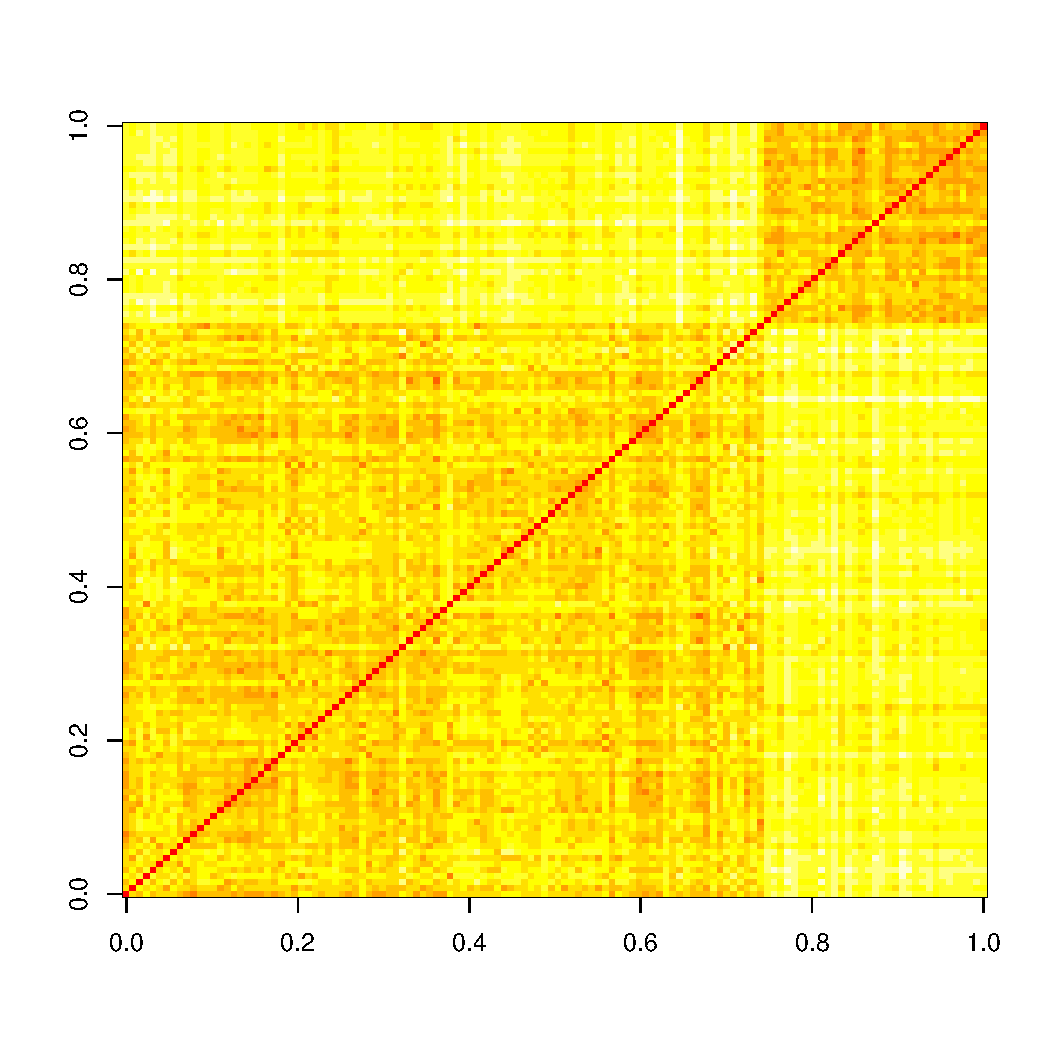
\includegraphics[width=.49\linewidth]{figure/hclust-plot-single-95-2-2} }\caption[based on Method]{based on Method: single, Filter: 95\%, Groups: 2}\label{fig:hclust-plot-single-95-2}
\end{figure}


\end{knitrout}


\begin{knitrout}
\definecolor{shadecolor}{rgb}{0.969, 0.969, 0.969}\color{fgcolor}\begin{figure}[H]

{\centering 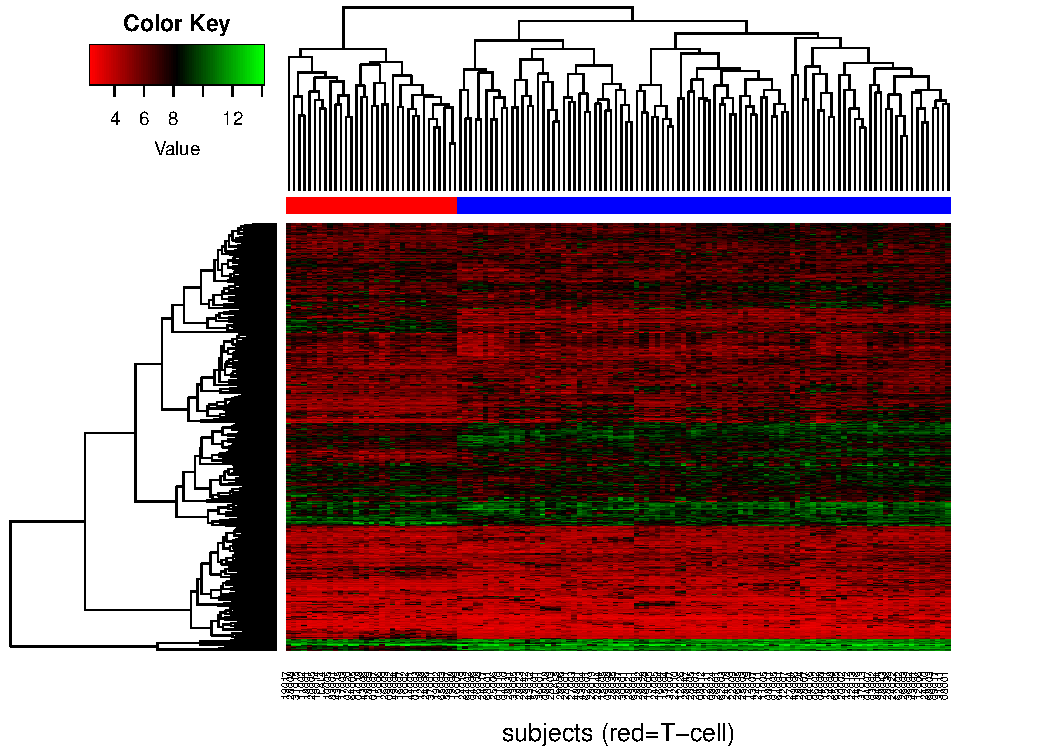
\includegraphics[width=\maxwidth]{figure/heatmap-single-95-2-1} 

}

\caption[Heatmap of Gene expression values for genes that survived a filter of 95\%]{Heatmap of Gene expression values for genes that survived a filter of 95\%}\label{fig:heatmap-single-95-2}
\end{figure}


\end{knitrout}


\newpage
\section{Method: complete, Filter: 95\%, Groups: 2}



\begin{knitrout}
\definecolor{shadecolor}{rgb}{0.969, 0.969, 0.969}\color{fgcolor}\begin{kframe}
\begin{alltt}
\hlkwd{dim}\hlstd{(dat.filter)}
\end{alltt}
\begin{verbatim}
## [1] 632 128
\end{verbatim}
\begin{alltt}
\hlkwd{table}\hlstd{(groups, cl)}
\end{alltt}
\begin{verbatim}
##       cl
## groups  B  T
##      1 95  0
##      2  0 33
\end{verbatim}
\begin{alltt}
\hlkwd{fisher.test}\hlstd{(groups, cl)}\hlopt{$}\hlstd{p.value}
\end{alltt}
\begin{verbatim}
## [1] 2.3e-31
\end{verbatim}
\end{kframe}
\end{knitrout}

\begin{knitrout}
\definecolor{shadecolor}{rgb}{0.969, 0.969, 0.969}\color{fgcolor}\begin{figure}[H]
\subfloat[Dendogram \label{fig:hclust-plot-complete-95-21}]{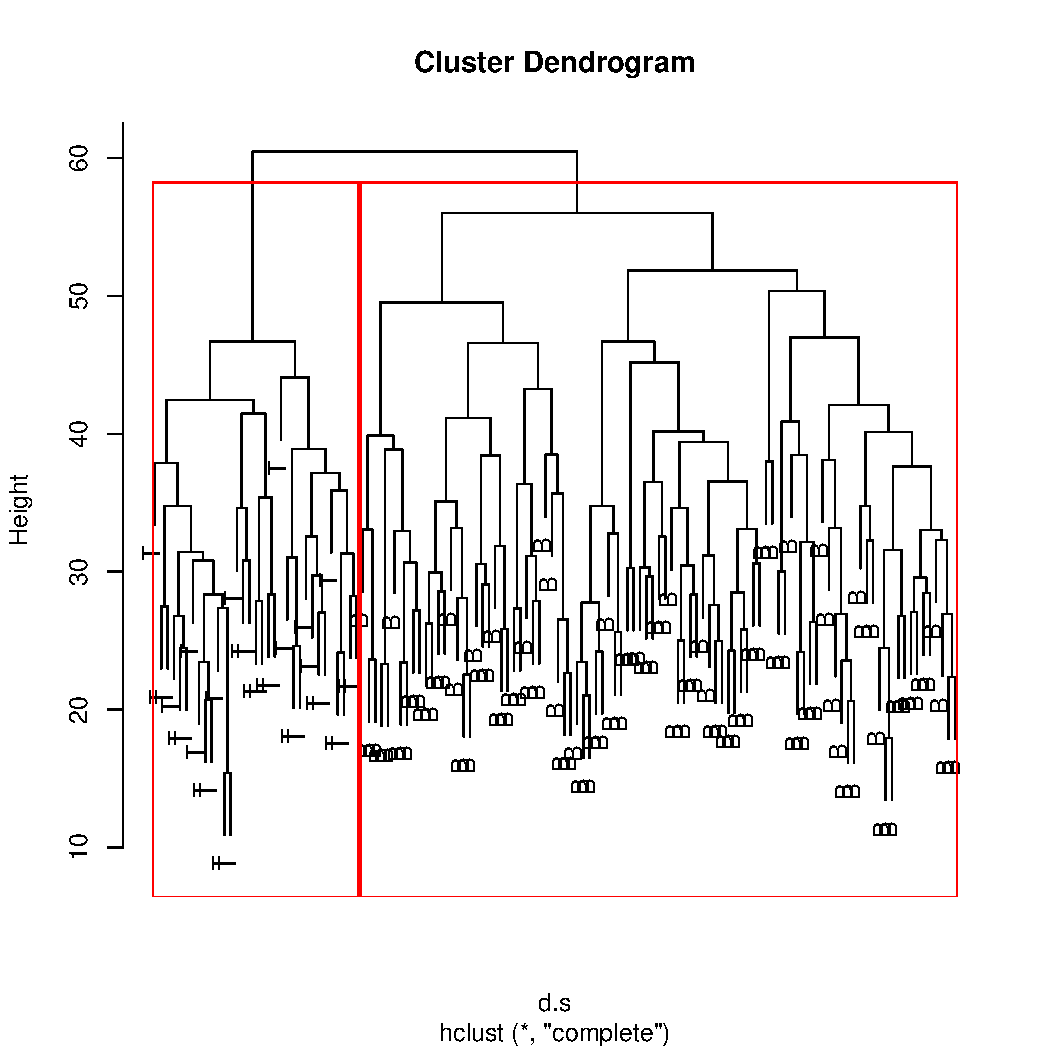
\includegraphics[width=.49\linewidth]{figure/hclust-plot-complete-95-2-1} }
\subfloat[Distance Matrix\label{fig:hclust-plot-complete-95-22}]{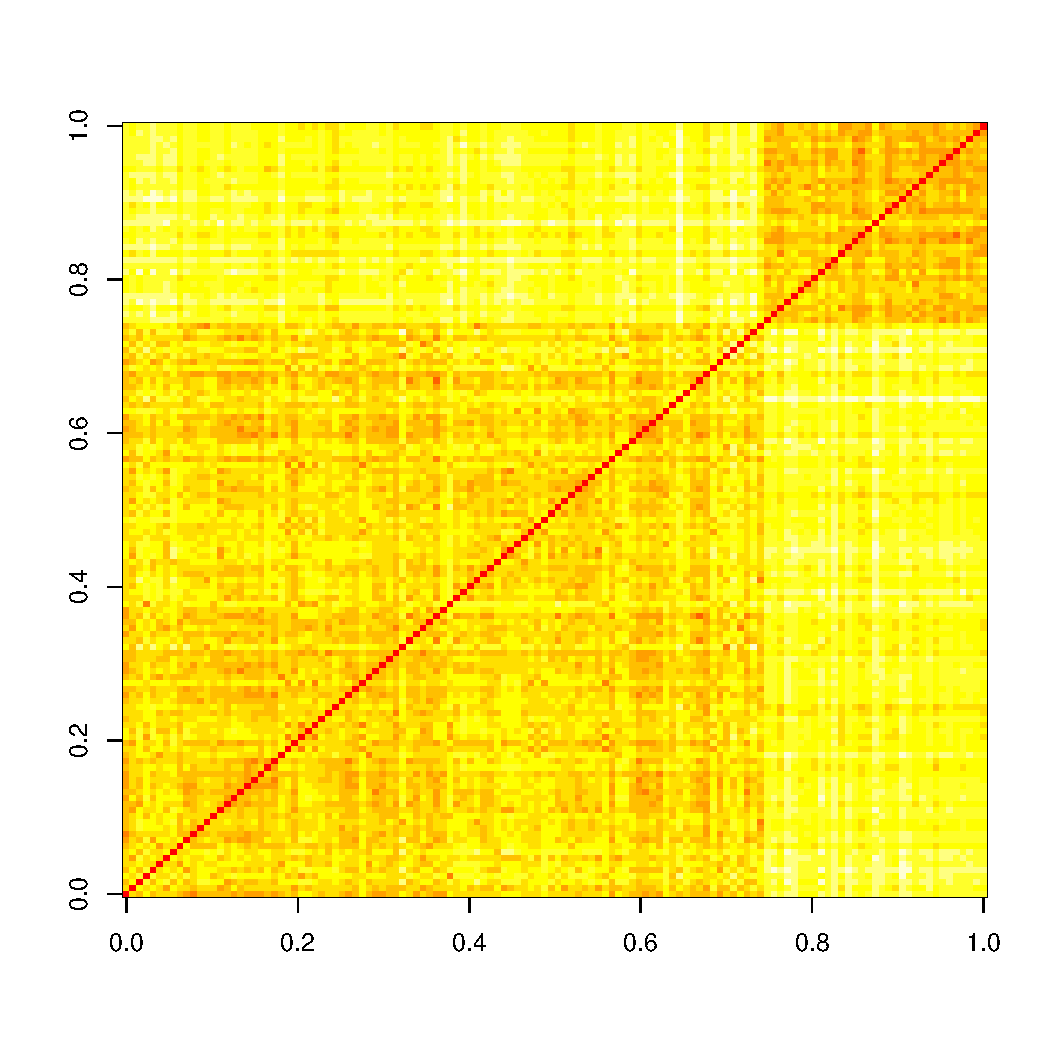
\includegraphics[width=.49\linewidth]{figure/hclust-plot-complete-95-2-2} }\caption[based on Method]{based on Method: complete, Filter: 95\%, Groups: 2}\label{fig:hclust-plot-complete-95-2}
\end{figure}


\end{knitrout}


\begin{knitrout}
\definecolor{shadecolor}{rgb}{0.969, 0.969, 0.969}\color{fgcolor}\begin{figure}[H]

{\centering 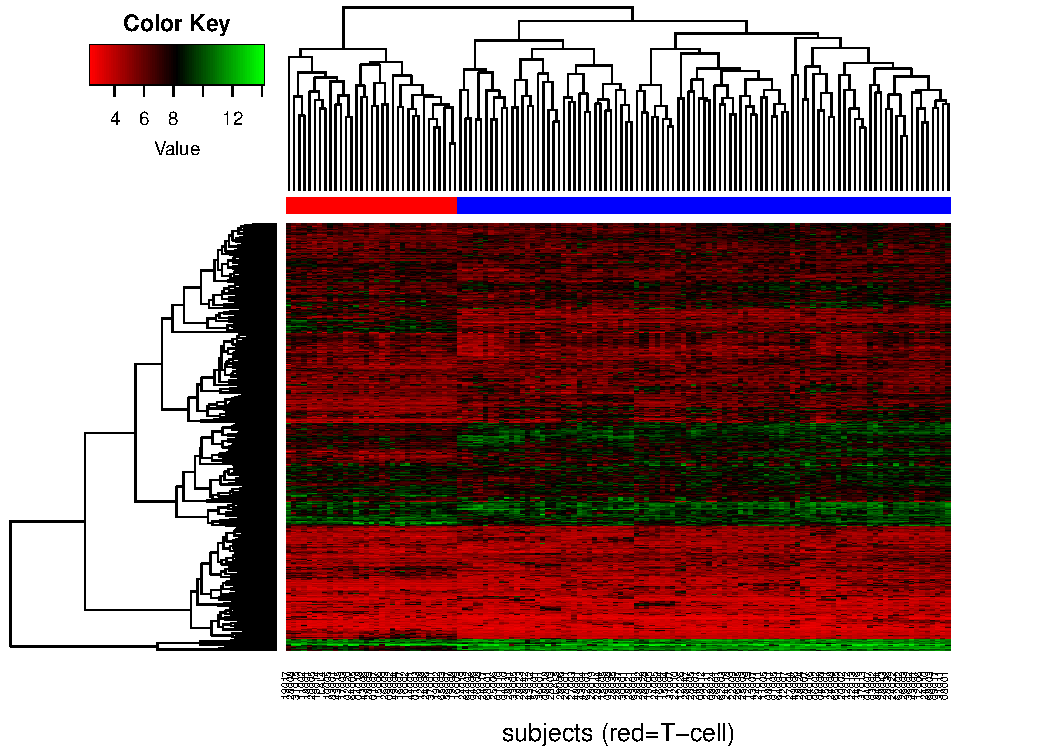
\includegraphics[width=\maxwidth]{figure/heatmap-complete-95-2-1} 

}

\caption[Heatmap of Gene expression values for genes that survived a filter of 95\%]{Heatmap of Gene expression values for genes that survived a filter of 95\%}\label{fig:heatmap-complete-95-2}
\end{figure}


\end{knitrout}


\newpage
\section{Method: average, Filter: 95\%, Groups: 2}



\begin{knitrout}
\definecolor{shadecolor}{rgb}{0.969, 0.969, 0.969}\color{fgcolor}\begin{kframe}
\begin{alltt}
\hlkwd{dim}\hlstd{(dat.filter)}
\end{alltt}
\begin{verbatim}
## [1] 632 128
\end{verbatim}
\begin{alltt}
\hlkwd{table}\hlstd{(groups, cl)}
\end{alltt}
\begin{verbatim}
##       cl
## groups  B  T
##      1 95  0
##      2  0 33
\end{verbatim}
\begin{alltt}
\hlkwd{fisher.test}\hlstd{(groups, cl)}\hlopt{$}\hlstd{p.value}
\end{alltt}
\begin{verbatim}
## [1] 2.3e-31
\end{verbatim}
\end{kframe}
\end{knitrout}

\begin{knitrout}
\definecolor{shadecolor}{rgb}{0.969, 0.969, 0.969}\color{fgcolor}\begin{figure}[H]
\subfloat[Dendogram \label{fig:hclust-plot-average-95-21}]{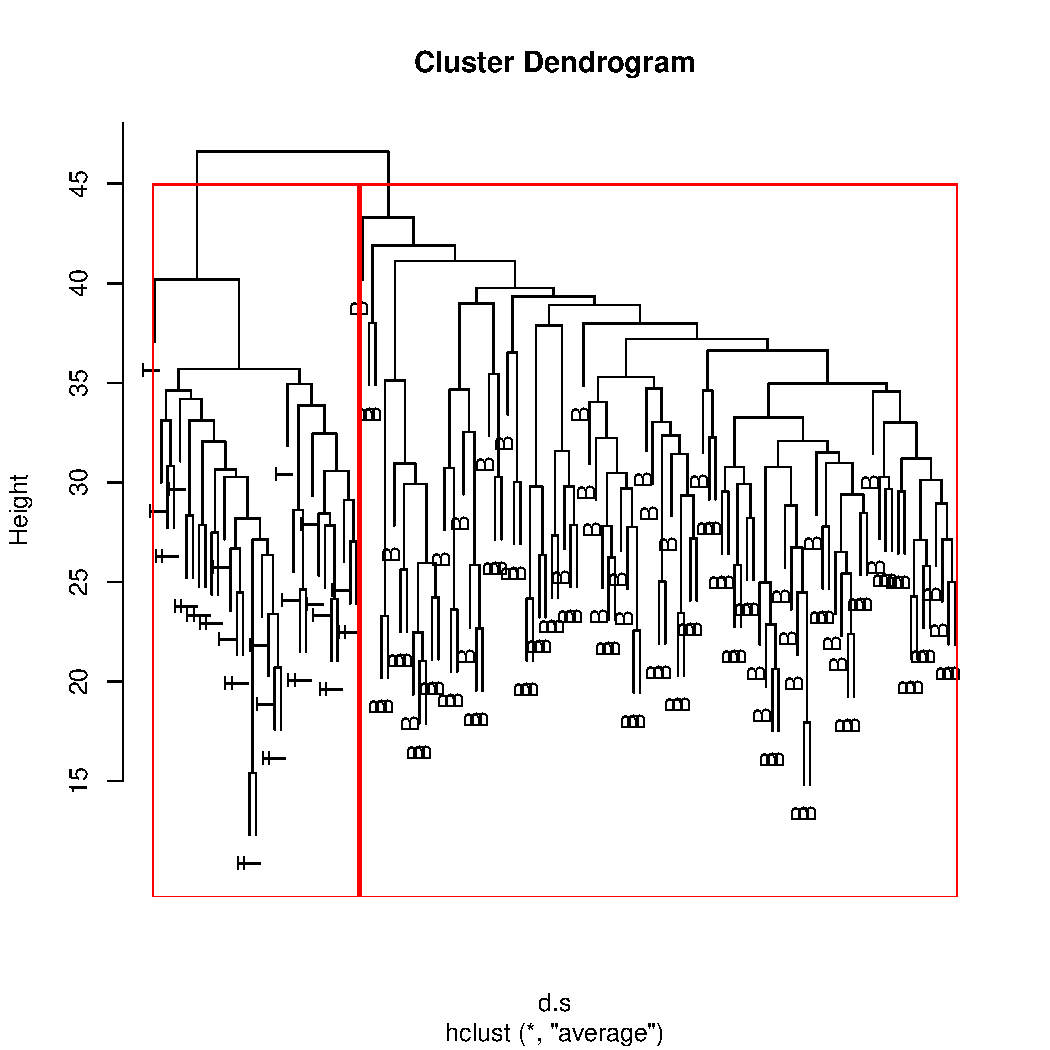
\includegraphics[width=.49\linewidth]{figure/hclust-plot-average-95-2-1} }
\subfloat[Distance Matrix\label{fig:hclust-plot-average-95-22}]{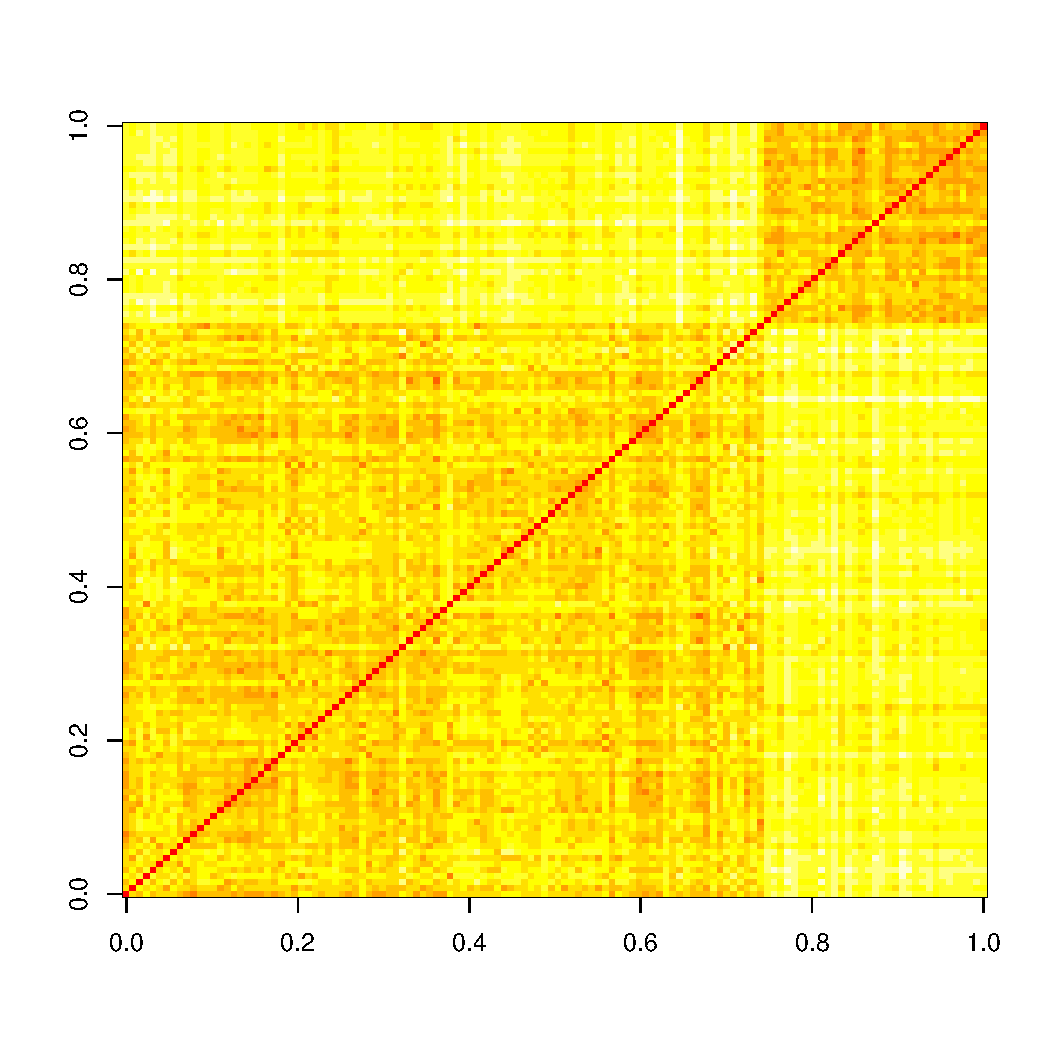
\includegraphics[width=.49\linewidth]{figure/hclust-plot-average-95-2-2} }\caption[based on Method]{based on Method: average, Filter: 95\%, Groups: 2}\label{fig:hclust-plot-average-95-2}
\end{figure}


\end{knitrout}


\begin{knitrout}
\definecolor{shadecolor}{rgb}{0.969, 0.969, 0.969}\color{fgcolor}\begin{figure}[H]

{\centering 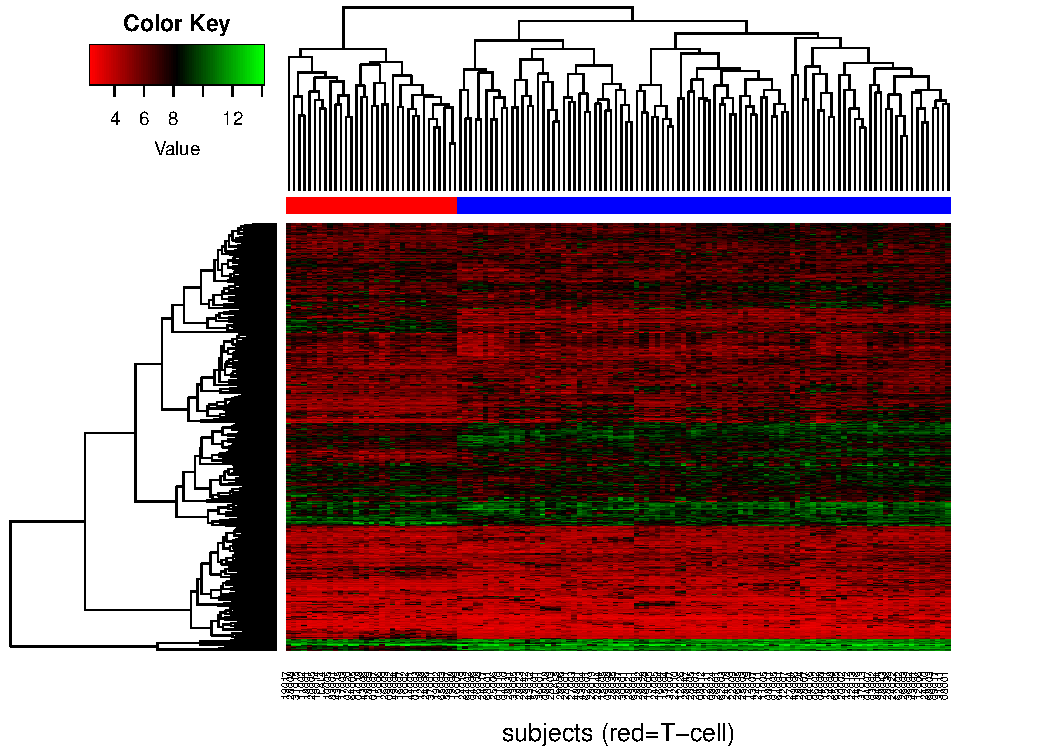
\includegraphics[width=\maxwidth]{figure/heatmap-average-95-2-1} 

}

\caption[Heatmap of Gene expression values for genes that survived a filter of 95\%]{Heatmap of Gene expression values for genes that survived a filter of 95\%}\label{fig:heatmap-average-95-2}
\end{figure}


\end{knitrout}


\newpage
\section{Method: mcquitty, Filter: 95\%, Groups: 2}



\begin{knitrout}
\definecolor{shadecolor}{rgb}{0.969, 0.969, 0.969}\color{fgcolor}\begin{kframe}
\begin{alltt}
\hlkwd{dim}\hlstd{(dat.filter)}
\end{alltt}
\begin{verbatim}
## [1] 632 128
\end{verbatim}
\begin{alltt}
\hlkwd{table}\hlstd{(groups, cl)}
\end{alltt}
\begin{verbatim}
##       cl
## groups  B  T
##      1 95  0
##      2  0 33
\end{verbatim}
\begin{alltt}
\hlkwd{fisher.test}\hlstd{(groups, cl)}\hlopt{$}\hlstd{p.value}
\end{alltt}
\begin{verbatim}
## [1] 2.3e-31
\end{verbatim}
\end{kframe}
\end{knitrout}

\begin{knitrout}
\definecolor{shadecolor}{rgb}{0.969, 0.969, 0.969}\color{fgcolor}\begin{figure}[H]
\subfloat[Dendogram \label{fig:hclust-plot-mcquitty-95-21}]{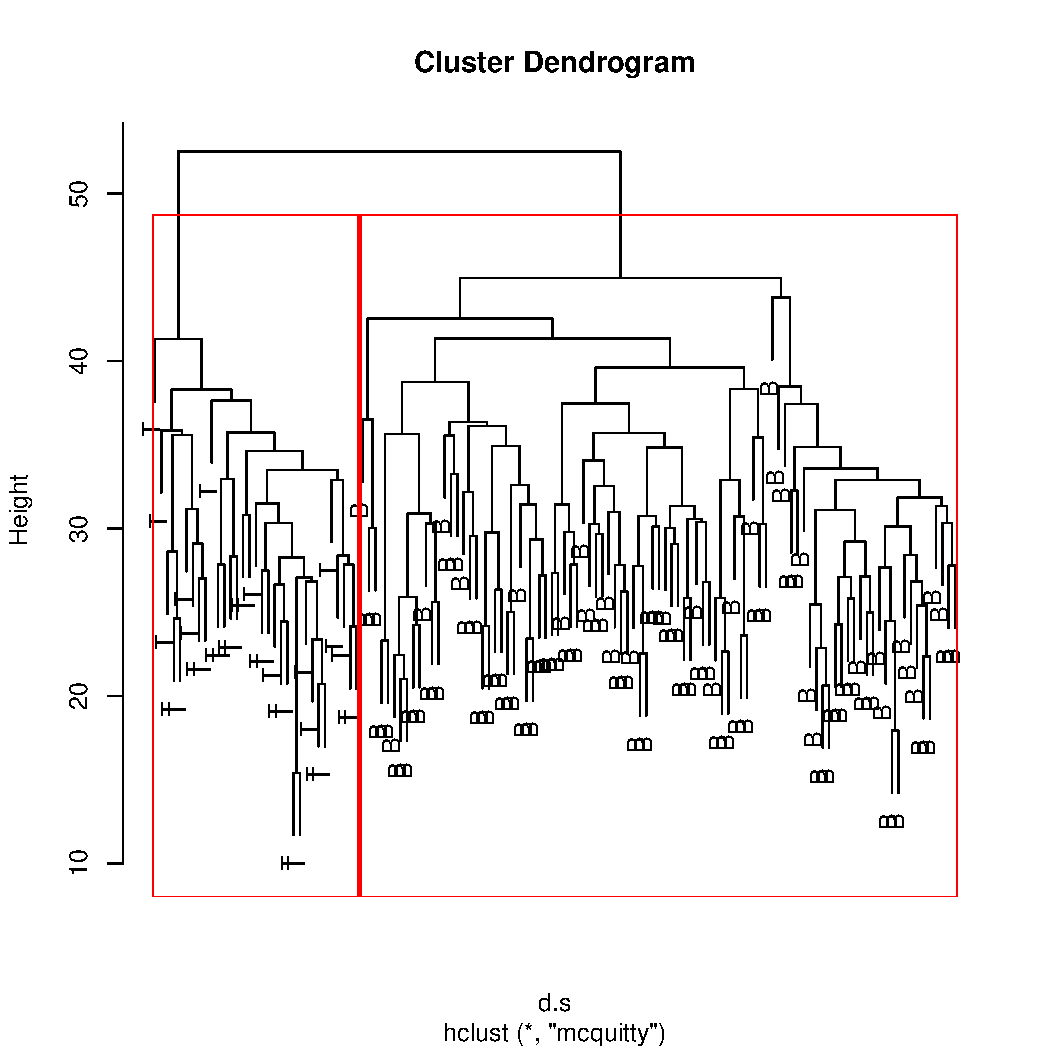
\includegraphics[width=.49\linewidth]{figure/hclust-plot-mcquitty-95-2-1} }
\subfloat[Distance Matrix\label{fig:hclust-plot-mcquitty-95-22}]{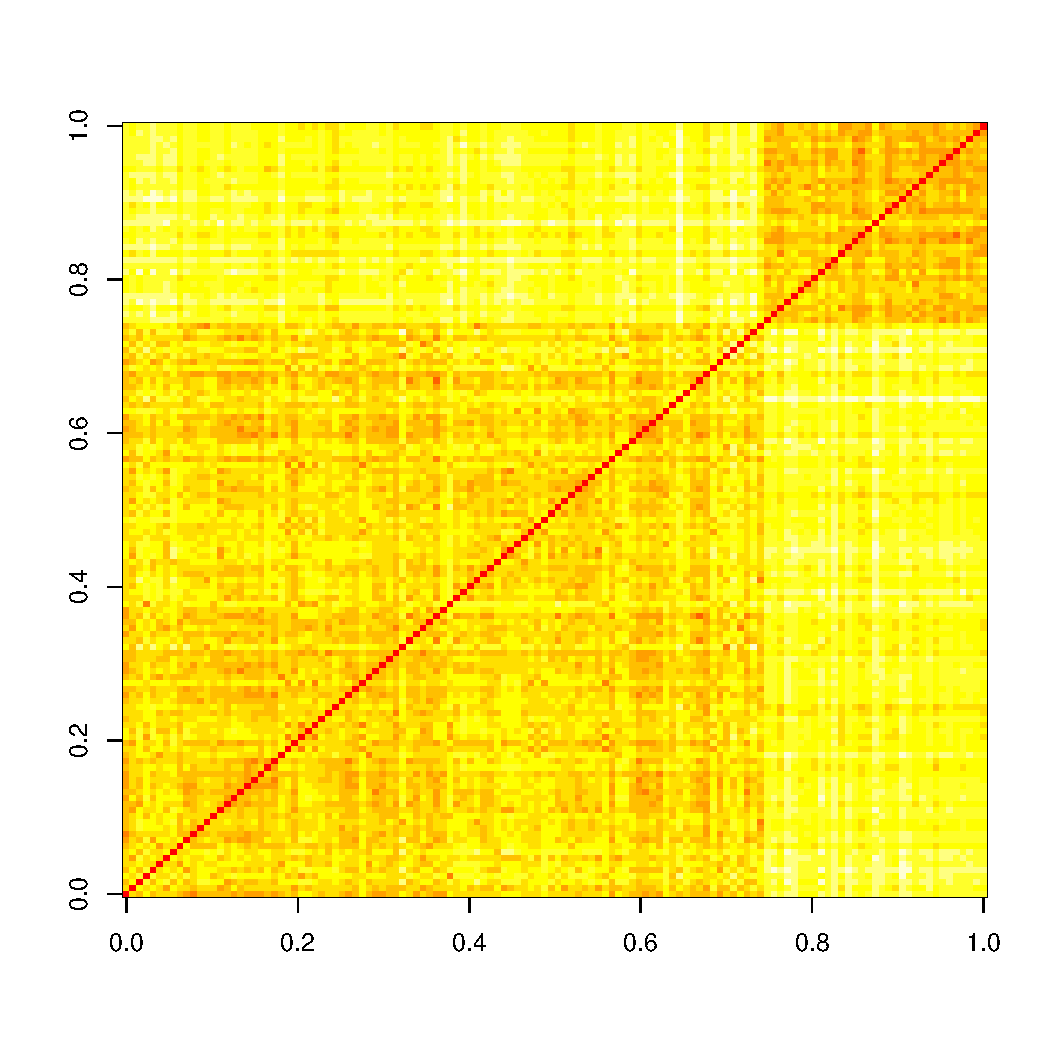
\includegraphics[width=.49\linewidth]{figure/hclust-plot-mcquitty-95-2-2} }\caption[based on Method]{based on Method: mcquitty, Filter: 95\%, Groups: 2}\label{fig:hclust-plot-mcquitty-95-2}
\end{figure}


\end{knitrout}


\begin{knitrout}
\definecolor{shadecolor}{rgb}{0.969, 0.969, 0.969}\color{fgcolor}\begin{figure}[H]

{\centering 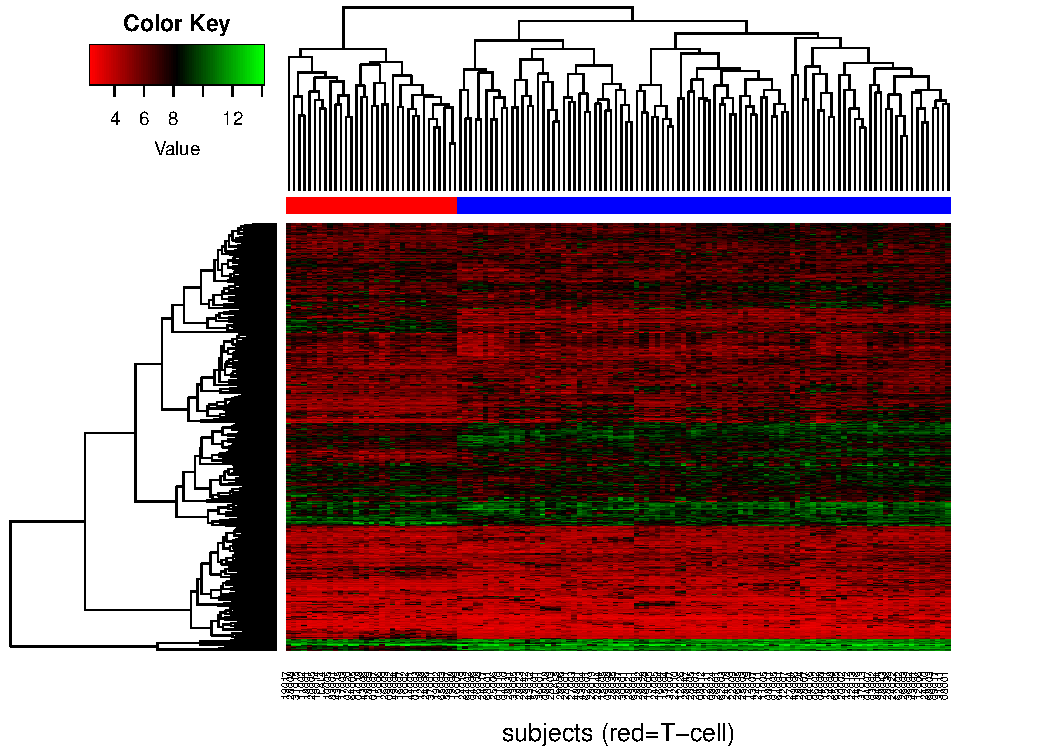
\includegraphics[width=\maxwidth]{figure/heatmap-mcquitty-95-2-1} 

}

\caption[Heatmap of Gene expression values for genes that survived a filter of 95\%]{Heatmap of Gene expression values for genes that survived a filter of 95\%}\label{fig:heatmap-mcquitty-95-2}
\end{figure}


\end{knitrout}


\newpage
\section{Method: median, Filter: 95\%, Groups: 2}



\begin{knitrout}
\definecolor{shadecolor}{rgb}{0.969, 0.969, 0.969}\color{fgcolor}\begin{kframe}
\begin{alltt}
\hlkwd{dim}\hlstd{(dat.filter)}
\end{alltt}
\begin{verbatim}
## [1] 632 128
\end{verbatim}
\begin{alltt}
\hlkwd{table}\hlstd{(groups, cl)}
\end{alltt}
\begin{verbatim}
##       cl
## groups  B  T
##      1 94 33
##      2  1  0
\end{verbatim}
\begin{alltt}
\hlkwd{fisher.test}\hlstd{(groups, cl)}\hlopt{$}\hlstd{p.value}
\end{alltt}
\begin{verbatim}
## [1] 1
\end{verbatim}
\end{kframe}
\end{knitrout}

\begin{knitrout}
\definecolor{shadecolor}{rgb}{0.969, 0.969, 0.969}\color{fgcolor}\begin{figure}[H]
\subfloat[Dendogram \label{fig:hclust-plot-median-95-21}]{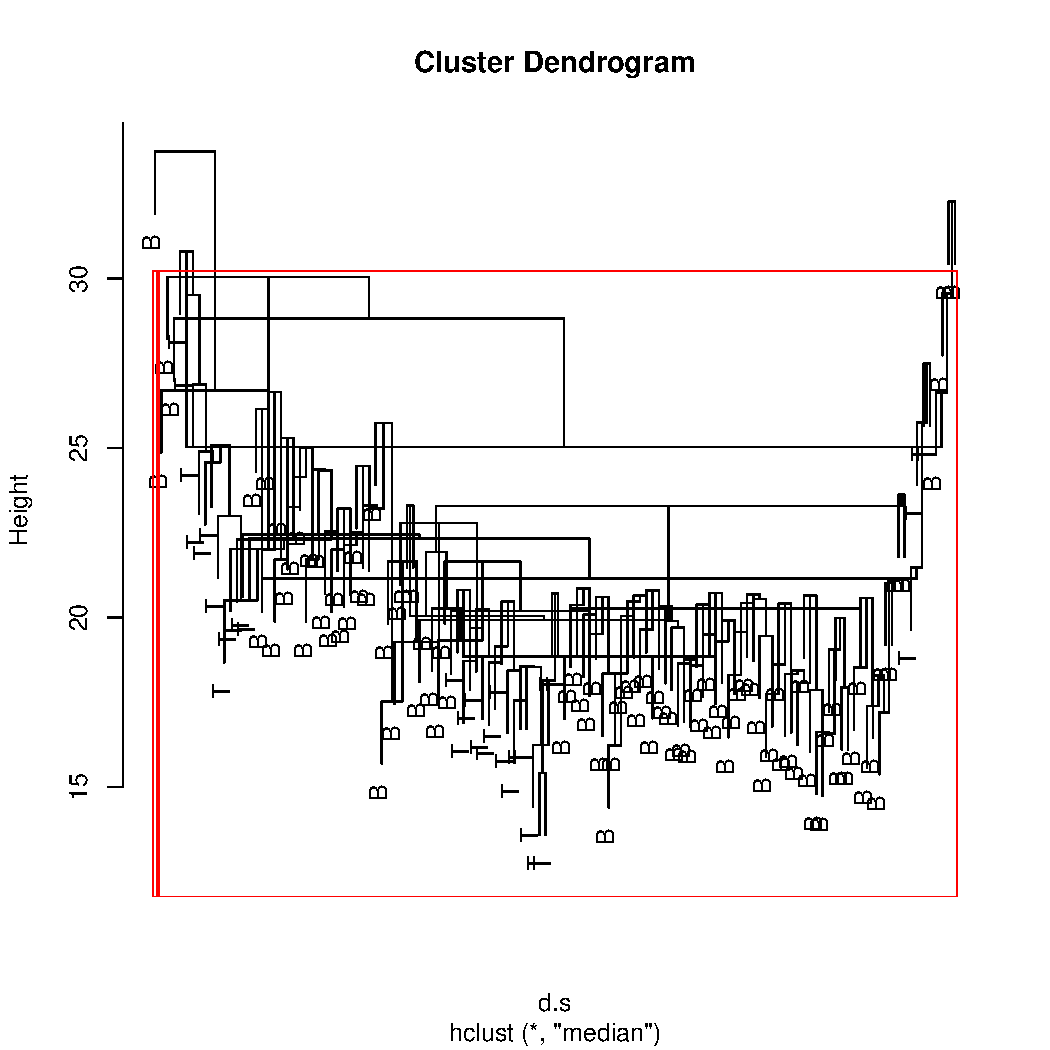
\includegraphics[width=.49\linewidth]{figure/hclust-plot-median-95-2-1} }
\subfloat[Distance Matrix\label{fig:hclust-plot-median-95-22}]{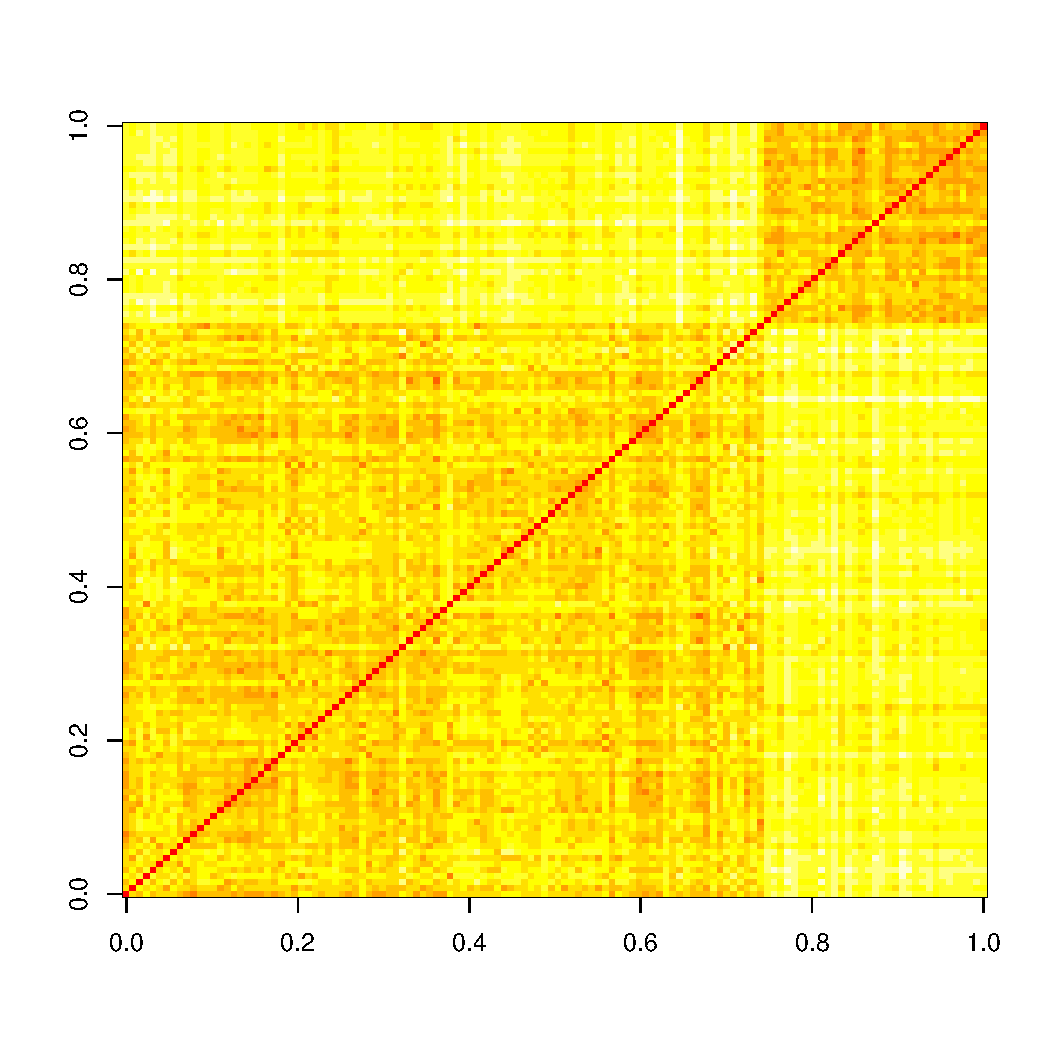
\includegraphics[width=.49\linewidth]{figure/hclust-plot-median-95-2-2} }\caption[based on Method]{based on Method: median, Filter: 95\%, Groups: 2}\label{fig:hclust-plot-median-95-2}
\end{figure}


\end{knitrout}


\begin{knitrout}
\definecolor{shadecolor}{rgb}{0.969, 0.969, 0.969}\color{fgcolor}\begin{figure}[H]

{\centering 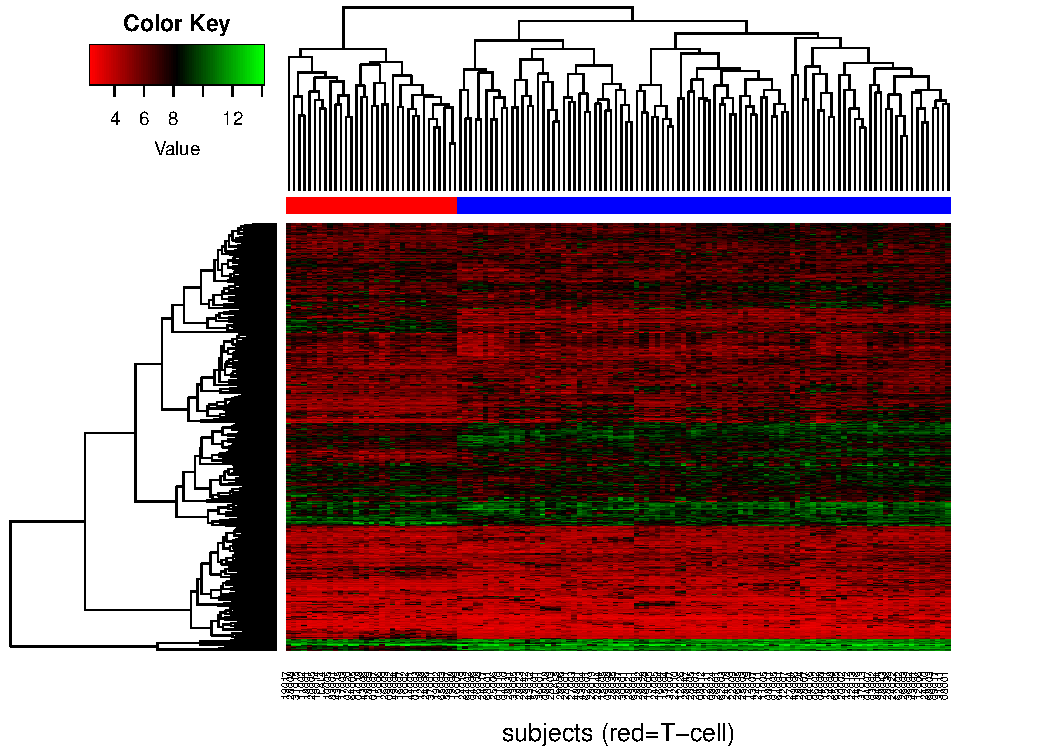
\includegraphics[width=\maxwidth]{figure/heatmap-median-95-2-1} 

}

\caption[Heatmap of Gene expression values for genes that survived a filter of 95\%]{Heatmap of Gene expression values for genes that survived a filter of 95\%}\label{fig:heatmap-median-95-2}
\end{figure}


\end{knitrout}


\newpage
\section{Method: centroid, Filter: 95\%, Groups: 2}



\begin{knitrout}
\definecolor{shadecolor}{rgb}{0.969, 0.969, 0.969}\color{fgcolor}\begin{kframe}
\begin{alltt}
\hlkwd{dim}\hlstd{(dat.filter)}
\end{alltt}
\begin{verbatim}
## [1] 632 128
\end{verbatim}
\begin{alltt}
\hlkwd{table}\hlstd{(groups, cl)}
\end{alltt}
\begin{verbatim}
##       cl
## groups  B  T
##      1 95 32
##      2  0  1
\end{verbatim}
\begin{alltt}
\hlkwd{fisher.test}\hlstd{(groups, cl)}\hlopt{$}\hlstd{p.value}
\end{alltt}
\begin{verbatim}
## [1] 0.26
\end{verbatim}
\end{kframe}
\end{knitrout}

\begin{knitrout}
\definecolor{shadecolor}{rgb}{0.969, 0.969, 0.969}\color{fgcolor}\begin{figure}[H]
\subfloat[Dendogram \label{fig:hclust-plot-centroid-95-21}]{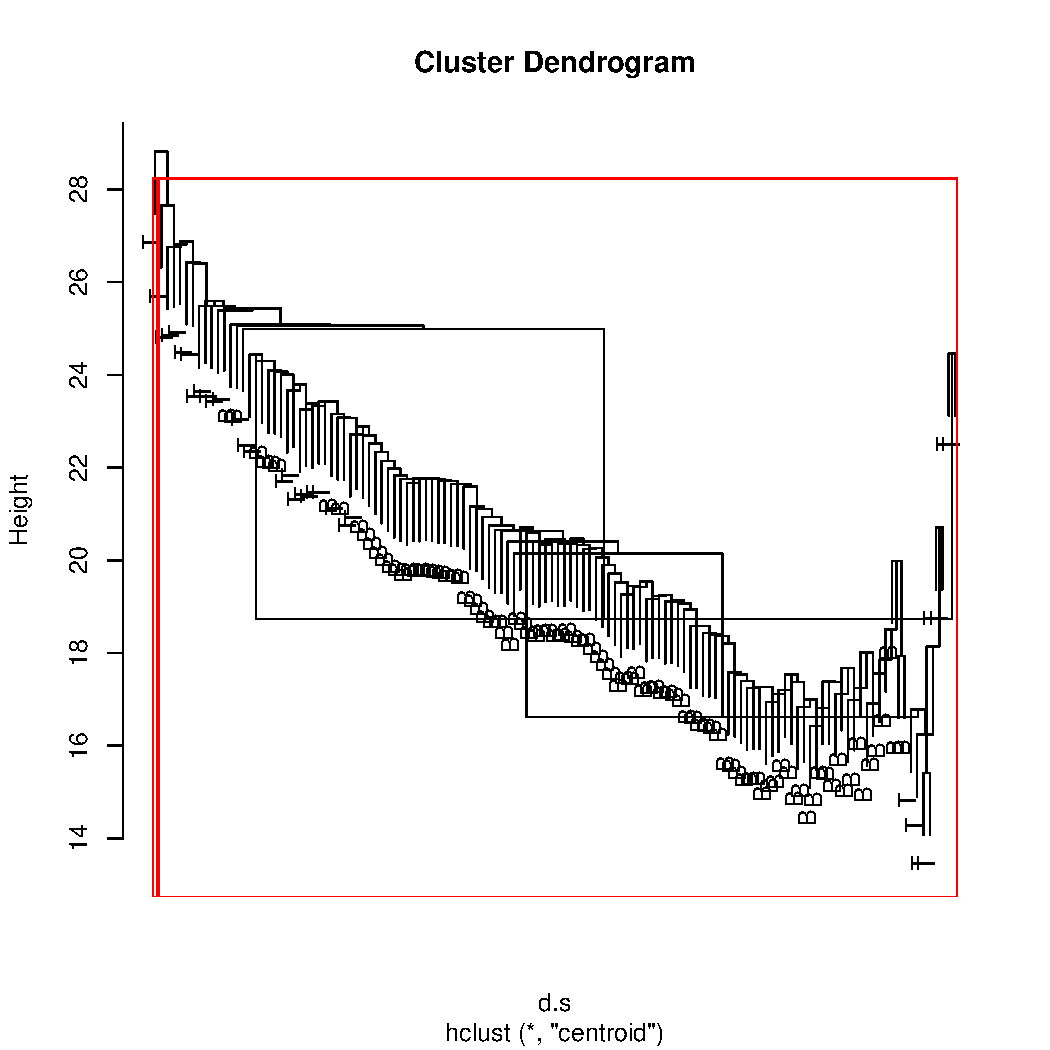
\includegraphics[width=.49\linewidth]{figure/hclust-plot-centroid-95-2-1} }
\subfloat[Distance Matrix\label{fig:hclust-plot-centroid-95-22}]{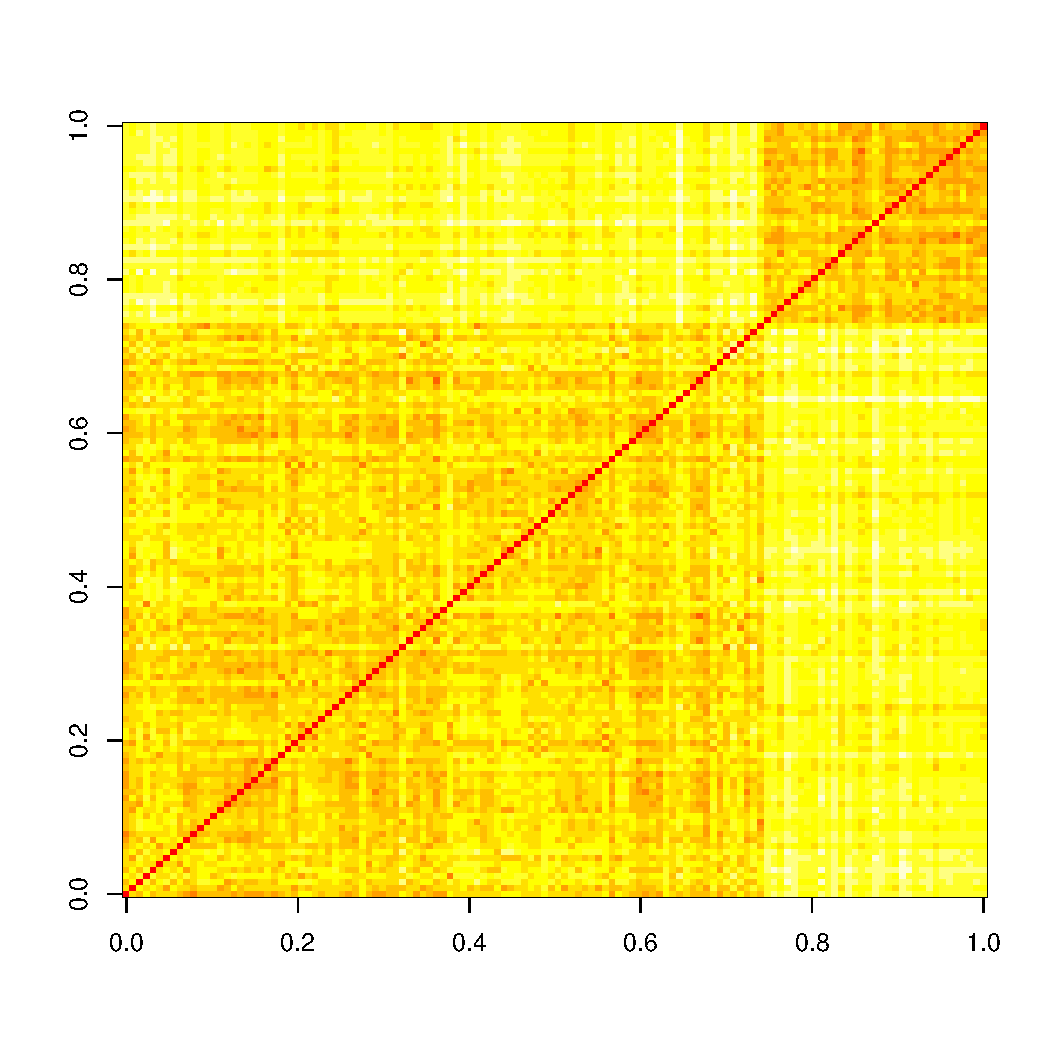
\includegraphics[width=.49\linewidth]{figure/hclust-plot-centroid-95-2-2} }\caption[based on Method]{based on Method: centroid, Filter: 95\%, Groups: 2}\label{fig:hclust-plot-centroid-95-2}
\end{figure}


\end{knitrout}


\begin{knitrout}
\definecolor{shadecolor}{rgb}{0.969, 0.969, 0.969}\color{fgcolor}\begin{figure}[H]

{\centering 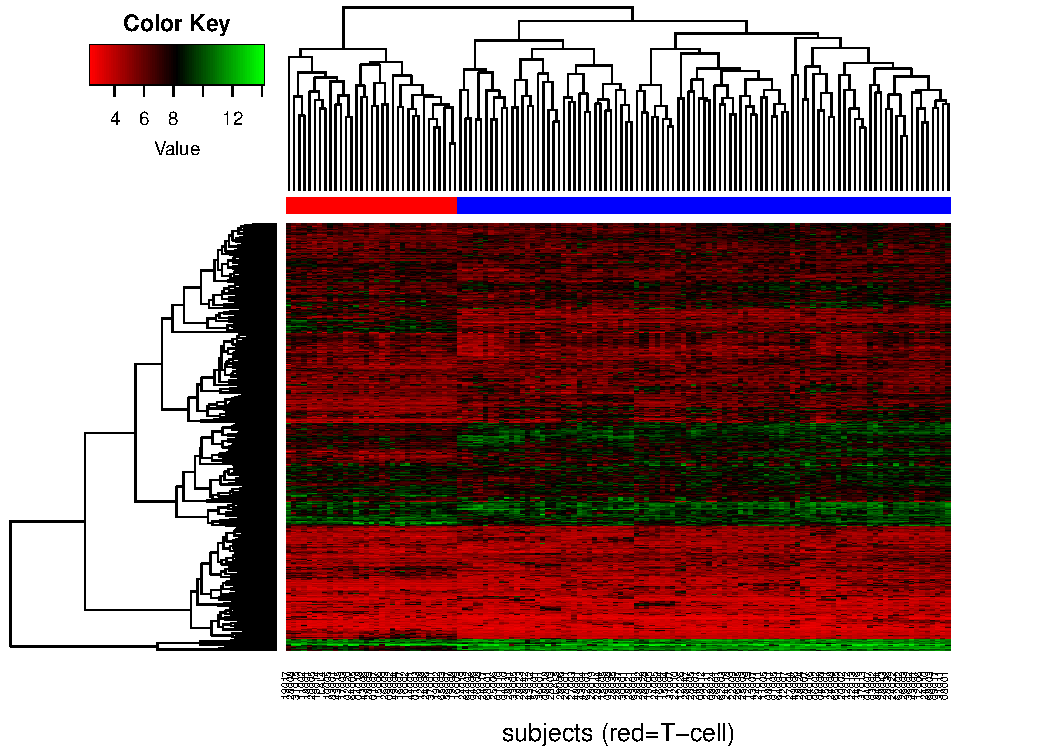
\includegraphics[width=\maxwidth]{figure/heatmap-centroid-95-2-1} 

}

\caption[Heatmap of Gene expression values for genes that survived a filter of 95\%]{Heatmap of Gene expression values for genes that survived a filter of 95\%}\label{fig:heatmap-centroid-95-2}
\end{figure}


\end{knitrout}




\FloatBarrier
\bibliography{007-bibliography}


\end{document}
